\section{FCCee: $e^{+}+e^{-}\rightarrow Z+H$ process }
\subsection{Event generator - PYTHIA8}

\begin{itemize}
\item To use Pythia8 we need a Gaudi steering file and a configuration file integrated in $Key4hep$ software stack. The steering file is a python script that is used to configure the Gaudi framework which runs Pythia8. The configuration file is a text file that is used to configure the Pythia8 generator. 
  
% \item We have selected Higgs-strahlung process $(e^{+} + e^{-} \longrightarrow Z + H)$ in production of Higgs by colliding $e^{+}$ and $e^{-}$ beams at center of mass energy $240$GeV.
\item In our case, data has been generated  by selecting Higgs production  $(HiggsSM:ffbar2HZ = on)$ in collision of  $e^{+}(Beams:idA = -11)$ and $e^{-}(Beams:idB = 11)$ collision at center of mass energy  $240$GeV. in pythia command file.



\begin{figure}[ht]
    \centering
    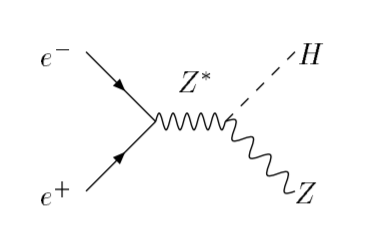
\includegraphics[scale= 0.9]{higgsprocess.png}
    \caption{Higgs-strahlung process}
    \label{fig:hsp}
\end{figure}



\item In  this cases 100000 will be generated and saved in 
ROOT files in $EDM4hep$ format. In order to get there we need 
first to generate the events in $HepMC$ format.

\item In order to get the events in $EDM4hep$ format, we will 
use Gaudi and the tools available in $k4FWCore$ and $k4Gen$. We 
need a Gaudi steering file that reads the $HepMC$ file and writes  out the $EDM4hep$ file format for later processing in $DDSim$.
\end{itemize}


\subsection{FCCee : Full simulation of CLD by DDSim}

\begin{itemize}
  \item We have set up the FCCSW software stack and used $DDSim$ to simulate the detector response of CLD by $/cvmfs/sw-nightlies.hsf.org/key4hep/setup.sh$.
  
  \item  The detectors in FCCSW are described in $DD4hep$ compact files. The compact files are written in XML and expose configuration options for the detector.
  
  \item Then run the simulation with detetor configuration file, event file and steering file and then run reconstruction. 
\end{itemize}

\subsection{Job submission in HTCondor batch system}
The CERN Batch Service is a fairly standard High Throughput Computing (HTC) Batch System with a fair-sharing mechanism.
Its purpose is to allow users to queue up jobs in the system, and maximise the utilisation of the batch farm.
\begin{figure}[h]
  \centering
  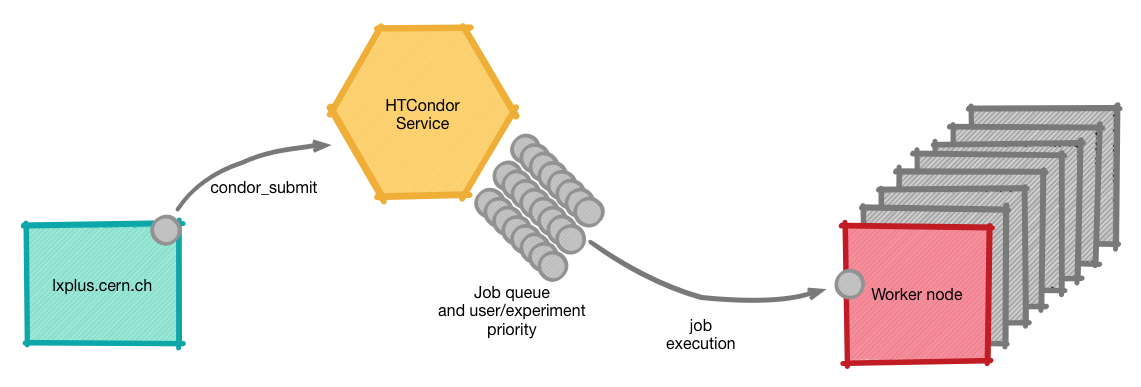
\includegraphics[width = 12cm, height = 4cm]{fcc_det/ex1.png}
  \caption{HTCondor}
  \label{fig:my_cond}
\end{figure}

Here we have submit our job to the batch system.The job is 
discrete and independent of other jobs. The job is submitted to 
the batch system and the batch system will run the job and 
return the output to the user. The batch system will also keep 
track of the jobs and their status.
\begin{itemize}
  \item HTCondor provides the ability to match executables files using regular expressions and add a job to the queue for each file. 
  \item In our case we have queued 10 jobs for respective $.sh$ executable file.The 10 jobs, even if they have different executables, have the same Cluster and different ProcIds.
\end{itemize}


\subsection{Analysis of Delphes samples$^{\cite{fcc}}$}
We have used Delphes sample  to get the detector response of CLD. Delphes is a fast detector 
simulation framework. It is based on the fast simulation package FastJet and uses the ROOT data 
analysis framework.
The FCCAnalyses framework is based on the RDataFrame interface which allows fast and efficient 
analysis of ROOT's TTrees and on samples following the $EDM4HEP$ event data model.
Here we have produced   flat ntuples with observables of interest and then 
produced plots with FCCAnalyses.
